% !TeX root = ../main.tex

\chapter{访问控制系统}

访问控制是计算机领域一个经典的问题,简单来说,计算机系统中的访问控制可以定义为防止对计算机中资源未授权的使用,包括未授权的用户对资源进行使用,或者对资源进行未授权的使用行为。访问控制系统用于管理数据的访问和操作权限,使得只有特定的用户才能进行特定的行为。传统的单机文件系统中通过对特定用户和用户组设置特定权限的方式进行文件权限的管理,而在分布式网络中,需要对不同的联网节点进行权限管理,到了互联网时代,网上应用的增加以及用户的多样化,对访问控制系统在安全性、灵活性等方面提出了更多的要求。

在互联网时代,网络中各平台分别管理用户的不同数据,为了提升易用性,方便第三方应用访问用户数据,OAuth框架被各大平台广泛应用。该框架中,主要有客户端,数据所有者,数据服务器和授权服务器四种角色,其中数据所有者将数据存储在数据服务器,给第三方客户端进行授权,客户端通过授权服务器换取凭证,用于访问数据服务器的数据。

\section{传统访问控制模型}

这一领域传统的访问控制模型主要有自主访问控制(Discretionary Access Control,DAC),强制访问控制(Mandatory Access Control,MAC),基于角色的访问控制(Role-Based Access Control,RBAC),基于属性的访问控制(Attribute-Based Access Control,ABAC),不同的模型都用于解决资源和用户之间连接关系的问题。

其中DAC模型基于以下概念:客体集合(即受保护的资源),一组主体(即一组访问权限定义了主体对某个对象(例如,读、写、执行等)的访问权限,以及一组可以用来表示约束的谓词。在访问控制矩阵中支持DAC存储访问规则的大多数系统。出于效率的考虑,访问控制矩阵按列存储(导致特定于对象的访问控制列表)或按行存储(导致特定于主题的功能列表)。主要应用于传统的单机文件系统。缺陷在于随着资源和用户数量的上升,访问控制列表的复杂度会急剧增加。

MAC模型对每个资源和每个用户设置等级,每个用户可以访问等级较低的资源,这一模型主要用于军队等资源等级明确的场景。

RBAC模型对不同的用户设置到各类角色,每一类角色拥有相同的权限,这一模型提升对一类用户修改权限以及对单一用户修改一类权限的效率。随着新的更灵活的权限范围不断出现,RBAC模型需要定义更多的角色。为了解决这一问题,ABAC模型将权限进一步细粒度化,对资源和角色都设定了一系列属性,通过属性访问控制列表对不同属性之间的关系进行管理。


由于在一个大组织或快速变化的环境中,创建和维护授权是一个动态复杂费时的任务,为了加入一个新用户,需要给该用户绑定所有需要的资源,直接将资源与用户绑定不仅费时,而且在用户任务变换的时候容易出错,比如忘了撤销某些权限。因此在RBAC模型中,角色是和具体用户无关的授权主体,包含完成该角色工作任务需要的权限。RBAC不允许用户直接和权限连接。先将权限授予角色,再将角色授予用户。两种不同的授权可以独立管理,并且很容易进行动态调整,方便管理。1996年,Sandhu等人将一般的RBAC分为四种概念模型。2000年,NIST开始建立RBAC的标准,并于2002年作为国际标准提交。

随着主体请求策略执行点(Policy Enforcement Point,PEP) 对资源进行访问,PEP 转发请求给策略判定点( Policy Decision Point,PDP) ,PDP 向主体属性权威( Subject Attribute Authority ) 、资 源 属 性 权 威 ( Resource Attribute Authority) 、环境属性权威( Environment Attribute Authority) 查询主体属性、客体属性、环境属性,并查询策略权威( Policy Authority) 判定访问的合法性,返回决策结果给 PEP 执行控制。


\section{OAuth 2.0框架}

近年来,用户数据逐渐集中存储在各大互联网公司的数据库中。用户希望能充分利用这些数据满足自身需求,为了缓解对公司自有解决方案的依赖,近年来出现了第三方独立服务提供商。第三方服务提供商通过获取用户授权,从大型公司的数据库中获取用户数据,为用户提供更丰富、灵活的服务。为了帮助大型公司管理第三方服务提供商对用户数据的访问,OAuth及类似的第三方授权协议被提出,OAuth协议在许多公司如Google和Facebook中被广泛使用。该协议可以支持细粒度、动态和灵活的特权管理,基于各种访问控制模型,如DAC(自主访问控制)、MAC(强制访问控制)、RBAC(基于角色的访问控制)和ABAC(基于属性的访问控制)。然而,第三方服务通常构建在集中的授权和身份验证系统上,容易受到来自内部和外部攻击的安全风险。例如,OAuth 2.0的不安全实现可能会导致重播攻击、模拟攻击、CSRF攻击等等。

\begin{figure}
\centering  
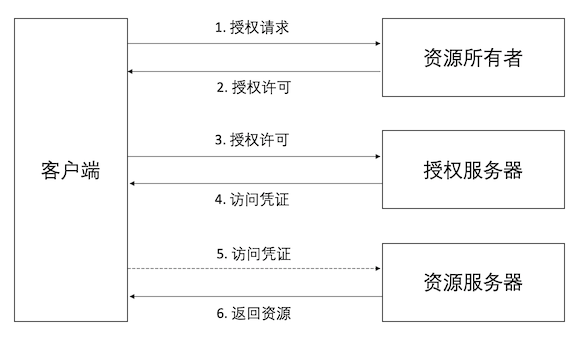
\includegraphics [width=400pt]{figures/oauth.pdf}
\caption{OAuth2.0协议中授权码模式的正常工作流程}
\label{fig:oauth}
\end{figure}

这里主要介绍OAuth 2.0框架中授权码模式的正常工作流程。如图\ref{fig:oauth}所示,该流程主要有以下3个阶段:

\begin{enumerate}
	\item 客户端向资源所有者发送授权请求,请求获取相应的资源访问权限。资源所有者收到请求和,检查请求的权限,通过验证后返回对应的授权许可给客户端。
	\item 客户端将授权许可发送给授权服务器,授权服务器验证后将对应资源的访问凭证返回给客户端。
	\item 客户端将访问凭证发送给资源服务器,资源服务器验证凭证后执行相应操作,并将结果返回给客户端。
\end{enumerate}

